% Created by tikzDevice version 0.7.0 on 2014-08-02 15:59:48
% !TEX encoding = UTF-8 Unicode
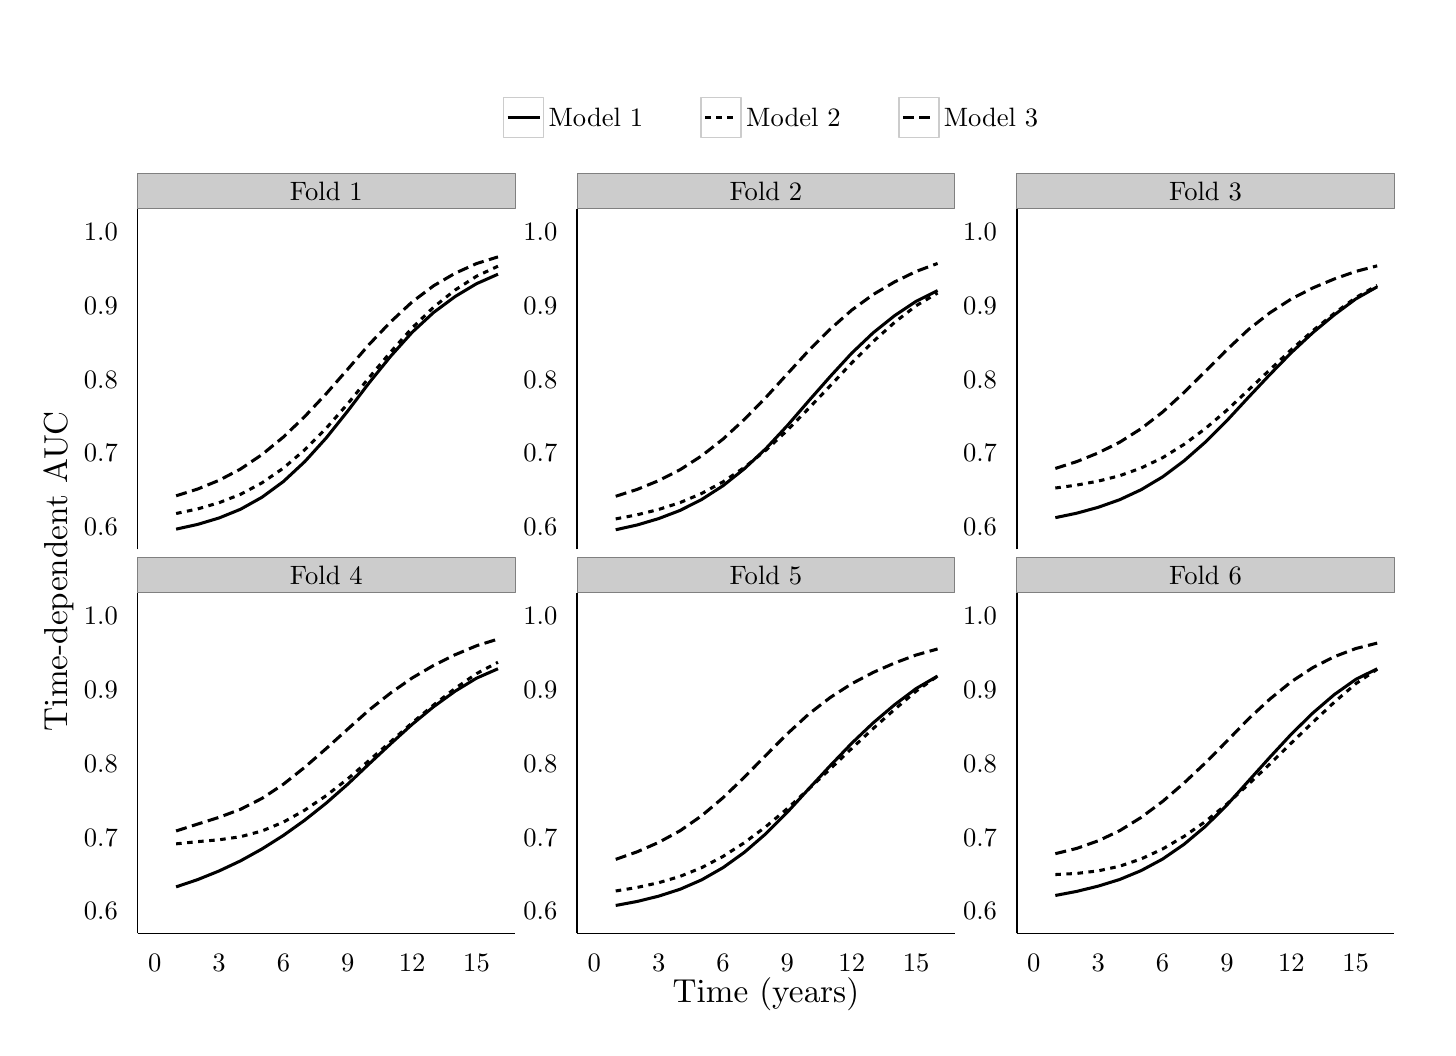
\begin{tikzpicture}[x=1pt,y=1pt]
\definecolor[named]{fillColor}{rgb}{1.00,1.00,1.00}
\path[use as bounding box,fill=fillColor,fill opacity=0.00] (0,0) rectangle (505.89,361.35);
\begin{scope}
\path[clip] (  0.00,  0.00) rectangle (505.89,361.35);
\definecolor[named]{drawColor}{rgb}{1.00,1.00,1.00}
\definecolor[named]{fillColor}{rgb}{1.00,1.00,1.00}

\path[draw=drawColor,line width= 0.6pt,line join=round,line cap=round,fill=fillColor] (  0.00,  0.00) rectangle (505.89,361.35);
\end{scope}
\begin{scope}
\path[clip] ( 39.69,172.81) rectangle (176.15,295.95);
\definecolor[named]{fillColor}{rgb}{1.00,1.00,1.00}

\path[fill=fillColor] ( 39.69,172.81) rectangle (176.15,295.95);
\definecolor[named]{drawColor}{rgb}{0.00,0.00,0.00}

\path[draw=drawColor,line width= 1.1pt,line join=round] ( 53.64,180.14) --
	( 61.40,181.85) --
	( 69.15,184.17) --
	( 76.90,187.32) --
	( 84.66,191.66) --
	( 92.41,197.35) --
	(100.16,204.57) --
	(107.92,213.14) --
	(115.67,222.84) --
	(123.42,233.06) --
	(131.18,242.63) --
	(138.93,251.27) --
	(146.68,258.43) --
	(154.44,264.18) --
	(162.19,268.83) --
	(169.94,272.26);

\path[draw=drawColor,line width= 1.1pt,dash pattern=on 2pt off 2pt ,line join=round] ( 53.64,185.79) --
	( 61.40,187.44) --
	( 69.15,189.69) --
	( 76.90,192.72) --
	( 84.66,196.86) --
	( 92.41,202.20) --
	(100.16,208.84) --
	(107.92,216.63) --
	(115.67,225.46) --
	(123.42,234.96) --
	(131.18,244.17) --
	(138.93,252.86) --
	(146.68,260.36) --
	(154.44,266.53) --
	(162.19,271.53) --
	(169.94,275.15);

\path[draw=drawColor,line width= 1.1pt,dash pattern=on 4pt off 2pt ,line join=round] ( 53.64,192.19) --
	( 61.40,194.62) --
	( 69.15,197.78) --
	( 76.90,201.85) --
	( 84.66,207.08) --
	( 92.41,213.43) --
	(100.16,220.87) --
	(107.92,229.13) --
	(115.67,237.97) --
	(123.42,246.92) --
	(131.18,255.06) --
	(138.93,262.25) --
	(146.68,268.08) --
	(154.44,272.60) --
	(162.19,276.10) --
	(169.94,278.52);
\end{scope}
\begin{scope}
\path[clip] (198.54,172.81) rectangle (335.00,295.95);
\definecolor[named]{fillColor}{rgb}{1.00,1.00,1.00}

\path[fill=fillColor] (198.54,172.81) rectangle (335.00,295.95);
\definecolor[named]{drawColor}{rgb}{0.00,0.00,0.00}

\path[draw=drawColor,line width= 1.1pt,line join=round] (212.49,179.92) --
	(220.25,181.65) --
	(228.00,183.95) --
	(235.75,186.91) --
	(243.51,190.83) --
	(251.26,195.82) --
	(259.01,202.00) --
	(266.77,209.26) --
	(274.52,217.58) --
	(282.27,226.53) --
	(290.03,235.33) --
	(297.78,243.75) --
	(305.53,251.11) --
	(313.29,257.32) --
	(321.04,262.47) --
	(328.79,266.35);

\path[draw=drawColor,line width= 1.1pt,dash pattern=on 2pt off 2pt ,line join=round] (212.49,183.84) --
	(220.25,185.32) --
	(228.00,187.25) --
	(235.75,189.74) --
	(243.51,193.02) --
	(251.26,197.24) --
	(259.01,202.47) --
	(266.77,208.68) --
	(274.52,215.88) --
	(282.27,223.83) --
	(290.03,231.97) --
	(297.78,240.22) --
	(305.53,247.94) --
	(313.29,254.88) --
	(321.04,260.88) --
	(328.79,265.46);

\path[draw=drawColor,line width= 1.1pt,dash pattern=on 4pt off 2pt ,line join=round] (212.49,192.02) --
	(220.25,194.50) --
	(228.00,197.67) --
	(235.75,201.61) --
	(243.51,206.61) --
	(251.26,212.68) --
	(259.01,219.83) --
	(266.77,227.76) --
	(274.52,236.26) --
	(282.27,244.74) --
	(290.03,252.45) --
	(297.78,259.30) --
	(305.53,264.93) --
	(313.29,269.50) --
	(321.04,273.26) --
	(328.79,276.15);
\end{scope}
\begin{scope}
\path[clip] (357.38,172.81) rectangle (493.85,295.95);
\definecolor[named]{fillColor}{rgb}{1.00,1.00,1.00}

\path[fill=fillColor] (357.38,172.81) rectangle (493.85,295.95);
\definecolor[named]{drawColor}{rgb}{0.00,0.00,0.00}

\path[draw=drawColor,line width= 1.1pt,line join=round] (371.34,184.29) --
	(379.09,185.91) --
	(386.85,188.04) --
	(394.60,190.78) --
	(402.35,194.40) --
	(410.11,199.03) --
	(417.86,204.82) --
	(425.61,211.64) --
	(433.37,219.39) --
	(441.12,227.77) --
	(448.88,236.01) --
	(456.63,243.94) --
	(464.38,251.13) --
	(472.14,257.57) --
	(479.89,263.31) --
	(487.64,267.71);

\path[draw=drawColor,line width= 1.1pt,dash pattern=on 2pt off 2pt ,line join=round] (371.34,195.00) --
	(379.09,196.06) --
	(386.85,197.49) --
	(394.60,199.45) --
	(402.35,202.23) --
	(410.11,205.96) --
	(417.86,210.77) --
	(425.61,216.53) --
	(433.37,223.15) --
	(441.12,230.42) --
	(448.88,237.74) --
	(456.63,245.02) --
	(464.38,251.83) --
	(472.14,258.11) --
	(479.89,263.80) --
	(487.64,268.22);

\path[draw=drawColor,line width= 1.1pt,dash pattern=on 4pt off 2pt ,line join=round] (371.34,202.07) --
	(379.09,204.55) --
	(386.85,207.69) --
	(394.60,211.55) --
	(402.35,216.45) --
	(410.11,222.45) --
	(417.86,229.54) --
	(425.61,237.23) --
	(433.37,245.00) --
	(441.12,252.27) --
	(448.88,258.33) --
	(456.63,263.33) --
	(464.38,267.30) --
	(472.14,270.54) --
	(479.89,273.26) --
	(487.64,275.28);
\end{scope}
\begin{scope}
\path[clip] ( 39.69, 34.03) rectangle (176.15,157.17);
\definecolor[named]{fillColor}{rgb}{1.00,1.00,1.00}

\path[fill=fillColor] ( 39.69, 34.03) rectangle (176.15,157.17);
\definecolor[named]{drawColor}{rgb}{0.00,0.00,0.00}

\path[draw=drawColor,line width= 1.1pt,line join=round] ( 53.64, 50.88) --
	( 61.40, 53.49) --
	( 69.15, 56.62) --
	( 76.90, 60.27) --
	( 84.66, 64.57) --
	( 92.41, 69.47) --
	(100.16, 75.01) --
	(107.92, 81.18) --
	(115.67, 87.99) --
	(123.42, 95.35) --
	(131.18,102.58) --
	(138.93,109.60) --
	(146.68,115.97) --
	(154.44,121.57) --
	(162.19,126.29) --
	(169.94,129.69);

\path[draw=drawColor,line width= 1.1pt,dash pattern=on 2pt off 2pt ,line join=round] ( 53.64, 66.42) --
	( 61.40, 67.22) --
	( 69.15, 67.89) --
	( 76.90, 69.00) --
	( 84.66, 71.07) --
	( 92.41, 74.28) --
	(100.16, 78.62) --
	(107.92, 83.89) --
	(115.67, 89.92) --
	(123.42, 96.60) --
	(131.18,103.35) --
	(138.93,110.15) --
	(146.68,116.59) --
	(154.44,122.58) --
	(162.19,127.93) --
	(169.94,132.05);

\path[draw=drawColor,line width= 1.1pt,dash pattern=on 4pt off 2pt ,line join=round] ( 53.64, 71.08) --
	( 61.40, 73.56) --
	( 69.15, 76.00) --
	( 76.90, 78.90) --
	( 84.66, 82.84) --
	( 92.41, 87.97) --
	(100.16, 94.13) --
	(107.92,100.90) --
	(115.67,107.91) --
	(123.42,114.83) --
	(131.18,120.95) --
	(138.93,126.36) --
	(146.68,130.90) --
	(154.44,134.75) --
	(162.19,138.00) --
	(169.94,140.42);
\end{scope}
\begin{scope}
\path[clip] (198.54, 34.03) rectangle (335.00,157.17);
\definecolor[named]{fillColor}{rgb}{1.00,1.00,1.00}

\path[fill=fillColor] (198.54, 34.03) rectangle (335.00,157.17);
\definecolor[named]{drawColor}{rgb}{0.00,0.00,0.00}

\path[draw=drawColor,line width= 1.1pt,line join=round] (212.49, 44.16) --
	(220.25, 45.61) --
	(228.00, 47.52) --
	(235.75, 50.02) --
	(243.51, 53.40) --
	(251.26, 57.82) --
	(259.01, 63.39) --
	(266.77, 70.11) --
	(274.52, 77.87) --
	(282.27, 86.33) --
	(290.03, 94.70) --
	(297.78,102.78) --
	(305.53,110.14) --
	(313.29,116.72) --
	(321.04,122.54) --
	(328.79,127.05);

\path[draw=drawColor,line width= 1.1pt,dash pattern=on 2pt off 2pt ,line join=round] (212.49, 49.39) --
	(220.25, 50.67) --
	(228.00, 52.38) --
	(235.75, 54.67) --
	(243.51, 57.81) --
	(251.26, 61.88) --
	(259.01, 66.86) --
	(266.77, 72.66) --
	(274.52, 79.18) --
	(282.27, 86.30) --
	(290.03, 93.53) --
	(297.78,100.91) --
	(305.53,108.10) --
	(313.29,115.03) --
	(321.04,121.59) --
	(328.79,127.03);

\path[draw=drawColor,line width= 1.1pt,dash pattern=on 4pt off 2pt ,line join=round] (212.49, 60.82) --
	(220.25, 63.55) --
	(228.00, 66.94) --
	(235.75, 71.16) --
	(243.51, 76.55) --
	(251.26, 83.09) --
	(259.01, 90.55) --
	(266.77, 98.45) --
	(274.52,106.22) --
	(282.27,113.36) --
	(290.03,119.32) --
	(297.78,124.30) --
	(305.53,128.37) --
	(313.29,131.78) --
	(321.04,134.66) --
	(328.79,136.85);
\end{scope}
\begin{scope}
\path[clip] (357.38, 34.03) rectangle (493.85,157.17);
\definecolor[named]{fillColor}{rgb}{1.00,1.00,1.00}

\path[fill=fillColor] (357.38, 34.03) rectangle (493.85,157.17);
\definecolor[named]{drawColor}{rgb}{0.00,0.00,0.00}

\path[draw=drawColor,line width= 1.1pt,line join=round] (371.34, 47.77) --
	(379.09, 49.25) --
	(386.85, 51.15) --
	(394.60, 53.55) --
	(402.35, 56.76) --
	(410.11, 60.93) --
	(417.86, 66.27) --
	(425.61, 72.77) --
	(433.37, 80.48) --
	(441.12, 89.12) --
	(448.88, 97.73) --
	(456.63,106.09) --
	(464.38,113.69) --
	(472.14,120.36) --
	(479.89,125.84) --
	(487.64,129.69);

\path[draw=drawColor,line width= 1.1pt,dash pattern=on 2pt off 2pt ,line join=round] (371.34, 55.33) --
	(379.09, 55.73) --
	(386.85, 56.67) --
	(394.60, 58.34) --
	(402.35, 60.98) --
	(410.11, 64.57) --
	(417.86, 69.12) --
	(425.61, 74.52) --
	(433.37, 80.83) --
	(441.12, 87.95) --
	(448.88, 95.29) --
	(456.63,102.87) --
	(464.38,110.35) --
	(472.14,117.60) --
	(479.89,124.28) --
	(487.64,129.51);

\path[draw=drawColor,line width= 1.1pt,dash pattern=on 4pt off 2pt ,line join=round] (371.34, 62.86) --
	(379.09, 64.78) --
	(386.85, 67.53) --
	(394.60, 71.18) --
	(402.35, 75.97) --
	(410.11, 81.75) --
	(417.86, 88.42) --
	(425.61, 95.72) --
	(433.37,103.57) --
	(441.12,111.55) --
	(448.88,118.75) --
	(456.63,125.03) --
	(464.38,130.10) --
	(472.14,134.05) --
	(479.89,136.99) --
	(487.64,138.96);
\end{scope}
\begin{scope}
\path[clip] (  0.00,  0.00) rectangle (505.89,361.35);
\definecolor[named]{drawColor}{rgb}{0.50,0.50,0.50}
\definecolor[named]{fillColor}{rgb}{0.80,0.80,0.80}

\path[draw=drawColor,line width= 0.2pt,line join=round,line cap=round,fill=fillColor] ( 39.69,295.95) rectangle (176.15,308.58);
\definecolor[named]{drawColor}{rgb}{0.00,0.00,0.00}

\node[text=drawColor,anchor=base,inner sep=0pt, outer sep=0pt, scale=  0.96] at (107.92,298.96) {Fold 1};
\end{scope}
\begin{scope}
\path[clip] (  0.00,  0.00) rectangle (505.89,361.35);
\definecolor[named]{drawColor}{rgb}{0.50,0.50,0.50}
\definecolor[named]{fillColor}{rgb}{0.80,0.80,0.80}

\path[draw=drawColor,line width= 0.2pt,line join=round,line cap=round,fill=fillColor] (198.54,295.95) rectangle (335.00,308.58);
\definecolor[named]{drawColor}{rgb}{0.00,0.00,0.00}

\node[text=drawColor,anchor=base,inner sep=0pt, outer sep=0pt, scale=  0.96] at (266.77,298.96) {Fold 2};
\end{scope}
\begin{scope}
\path[clip] (  0.00,  0.00) rectangle (505.89,361.35);
\definecolor[named]{drawColor}{rgb}{0.50,0.50,0.50}
\definecolor[named]{fillColor}{rgb}{0.80,0.80,0.80}

\path[draw=drawColor,line width= 0.2pt,line join=round,line cap=round,fill=fillColor] (357.38,295.95) rectangle (493.85,308.58);
\definecolor[named]{drawColor}{rgb}{0.00,0.00,0.00}

\node[text=drawColor,anchor=base,inner sep=0pt, outer sep=0pt, scale=  0.96] at (425.61,298.96) {Fold 3};
\end{scope}
\begin{scope}
\path[clip] (  0.00,  0.00) rectangle (505.89,361.35);
\definecolor[named]{drawColor}{rgb}{0.50,0.50,0.50}
\definecolor[named]{fillColor}{rgb}{0.80,0.80,0.80}

\path[draw=drawColor,line width= 0.2pt,line join=round,line cap=round,fill=fillColor] ( 39.69,157.17) rectangle (176.15,169.80);
\definecolor[named]{drawColor}{rgb}{0.00,0.00,0.00}

\node[text=drawColor,anchor=base,inner sep=0pt, outer sep=0pt, scale=  0.96] at (107.92,160.18) {Fold 4};
\end{scope}
\begin{scope}
\path[clip] (  0.00,  0.00) rectangle (505.89,361.35);
\definecolor[named]{drawColor}{rgb}{0.50,0.50,0.50}
\definecolor[named]{fillColor}{rgb}{0.80,0.80,0.80}

\path[draw=drawColor,line width= 0.2pt,line join=round,line cap=round,fill=fillColor] (198.54,157.17) rectangle (335.00,169.80);
\definecolor[named]{drawColor}{rgb}{0.00,0.00,0.00}

\node[text=drawColor,anchor=base,inner sep=0pt, outer sep=0pt, scale=  0.96] at (266.77,160.18) {Fold 5};
\end{scope}
\begin{scope}
\path[clip] (  0.00,  0.00) rectangle (505.89,361.35);
\definecolor[named]{drawColor}{rgb}{0.50,0.50,0.50}
\definecolor[named]{fillColor}{rgb}{0.80,0.80,0.80}

\path[draw=drawColor,line width= 0.2pt,line join=round,line cap=round,fill=fillColor] (357.38,157.17) rectangle (493.85,169.80);
\definecolor[named]{drawColor}{rgb}{0.00,0.00,0.00}

\node[text=drawColor,anchor=base,inner sep=0pt, outer sep=0pt, scale=  0.96] at (425.61,160.18) {Fold 6};
\end{scope}
\begin{scope}
\path[clip] (  0.00,  0.00) rectangle (505.89,361.35);
\definecolor[named]{drawColor}{rgb}{0.00,0.00,0.00}

\path[draw=drawColor,line width= 0.6pt,line join=round] ( 39.69,172.81) --
	( 39.69,295.95);
\end{scope}
\begin{scope}
\path[clip] (  0.00,  0.00) rectangle (505.89,361.35);
\definecolor[named]{drawColor}{rgb}{0.00,0.00,0.00}

\node[text=drawColor,anchor=base east,inner sep=0pt, outer sep=0pt, scale=  0.96] at ( 32.57,177.77) {0.6};

\node[text=drawColor,anchor=base east,inner sep=0pt, outer sep=0pt, scale=  0.96] at ( 32.57,204.42) {0.7};

\node[text=drawColor,anchor=base east,inner sep=0pt, outer sep=0pt, scale=  0.96] at ( 32.57,231.07) {0.8};

\node[text=drawColor,anchor=base east,inner sep=0pt, outer sep=0pt, scale=  0.96] at ( 32.57,257.73) {0.9};

\node[text=drawColor,anchor=base east,inner sep=0pt, outer sep=0pt, scale=  0.96] at ( 32.57,284.38) {1.0};
\end{scope}
\begin{scope}
\path[clip] (  0.00,  0.00) rectangle (505.89,361.35);
\definecolor[named]{drawColor}{rgb}{0.00,0.00,0.00}

\path[draw=drawColor,line width= 0.6pt,line join=round] (198.54,172.81) --
	(198.54,295.95);
\end{scope}
\begin{scope}
\path[clip] (  0.00,  0.00) rectangle (505.89,361.35);
\definecolor[named]{drawColor}{rgb}{0.00,0.00,0.00}

\node[text=drawColor,anchor=base east,inner sep=0pt, outer sep=0pt, scale=  0.96] at (191.42,177.77) {0.6};

\node[text=drawColor,anchor=base east,inner sep=0pt, outer sep=0pt, scale=  0.96] at (191.42,204.42) {0.7};

\node[text=drawColor,anchor=base east,inner sep=0pt, outer sep=0pt, scale=  0.96] at (191.42,231.07) {0.8};

\node[text=drawColor,anchor=base east,inner sep=0pt, outer sep=0pt, scale=  0.96] at (191.42,257.73) {0.9};

\node[text=drawColor,anchor=base east,inner sep=0pt, outer sep=0pt, scale=  0.96] at (191.42,284.38) {1.0};
\end{scope}
\begin{scope}
\path[clip] (  0.00,  0.00) rectangle (505.89,361.35);
\definecolor[named]{drawColor}{rgb}{0.00,0.00,0.00}

\path[draw=drawColor,line width= 0.6pt,line join=round] (357.38,172.81) --
	(357.38,295.95);
\end{scope}
\begin{scope}
\path[clip] (  0.00,  0.00) rectangle (505.89,361.35);
\definecolor[named]{drawColor}{rgb}{0.00,0.00,0.00}

\node[text=drawColor,anchor=base east,inner sep=0pt, outer sep=0pt, scale=  0.96] at (350.27,177.77) {0.6};

\node[text=drawColor,anchor=base east,inner sep=0pt, outer sep=0pt, scale=  0.96] at (350.27,204.42) {0.7};

\node[text=drawColor,anchor=base east,inner sep=0pt, outer sep=0pt, scale=  0.96] at (350.27,231.07) {0.8};

\node[text=drawColor,anchor=base east,inner sep=0pt, outer sep=0pt, scale=  0.96] at (350.27,257.73) {0.9};

\node[text=drawColor,anchor=base east,inner sep=0pt, outer sep=0pt, scale=  0.96] at (350.27,284.38) {1.0};
\end{scope}
\begin{scope}
\path[clip] (  0.00,  0.00) rectangle (505.89,361.35);
\definecolor[named]{drawColor}{rgb}{0.00,0.00,0.00}

\path[draw=drawColor,line width= 0.6pt,line join=round] ( 39.69, 34.03) --
	( 39.69,157.17);
\end{scope}
\begin{scope}
\path[clip] (  0.00,  0.00) rectangle (505.89,361.35);
\definecolor[named]{drawColor}{rgb}{0.00,0.00,0.00}

\node[text=drawColor,anchor=base east,inner sep=0pt, outer sep=0pt, scale=  0.96] at ( 32.57, 38.99) {0.6};

\node[text=drawColor,anchor=base east,inner sep=0pt, outer sep=0pt, scale=  0.96] at ( 32.57, 65.64) {0.7};

\node[text=drawColor,anchor=base east,inner sep=0pt, outer sep=0pt, scale=  0.96] at ( 32.57, 92.30) {0.8};

\node[text=drawColor,anchor=base east,inner sep=0pt, outer sep=0pt, scale=  0.96] at ( 32.57,118.95) {0.9};

\node[text=drawColor,anchor=base east,inner sep=0pt, outer sep=0pt, scale=  0.96] at ( 32.57,145.60) {1.0};
\end{scope}
\begin{scope}
\path[clip] (  0.00,  0.00) rectangle (505.89,361.35);
\definecolor[named]{drawColor}{rgb}{0.00,0.00,0.00}

\path[draw=drawColor,line width= 0.6pt,line join=round] (198.54, 34.03) --
	(198.54,157.17);
\end{scope}
\begin{scope}
\path[clip] (  0.00,  0.00) rectangle (505.89,361.35);
\definecolor[named]{drawColor}{rgb}{0.00,0.00,0.00}

\node[text=drawColor,anchor=base east,inner sep=0pt, outer sep=0pt, scale=  0.96] at (191.42, 38.99) {0.6};

\node[text=drawColor,anchor=base east,inner sep=0pt, outer sep=0pt, scale=  0.96] at (191.42, 65.64) {0.7};

\node[text=drawColor,anchor=base east,inner sep=0pt, outer sep=0pt, scale=  0.96] at (191.42, 92.30) {0.8};

\node[text=drawColor,anchor=base east,inner sep=0pt, outer sep=0pt, scale=  0.96] at (191.42,118.95) {0.9};

\node[text=drawColor,anchor=base east,inner sep=0pt, outer sep=0pt, scale=  0.96] at (191.42,145.60) {1.0};
\end{scope}
\begin{scope}
\path[clip] (  0.00,  0.00) rectangle (505.89,361.35);
\definecolor[named]{drawColor}{rgb}{0.00,0.00,0.00}

\path[draw=drawColor,line width= 0.6pt,line join=round] (357.38, 34.03) --
	(357.38,157.17);
\end{scope}
\begin{scope}
\path[clip] (  0.00,  0.00) rectangle (505.89,361.35);
\definecolor[named]{drawColor}{rgb}{0.00,0.00,0.00}

\node[text=drawColor,anchor=base east,inner sep=0pt, outer sep=0pt, scale=  0.96] at (350.27, 38.99) {0.6};

\node[text=drawColor,anchor=base east,inner sep=0pt, outer sep=0pt, scale=  0.96] at (350.27, 65.64) {0.7};

\node[text=drawColor,anchor=base east,inner sep=0pt, outer sep=0pt, scale=  0.96] at (350.27, 92.30) {0.8};

\node[text=drawColor,anchor=base east,inner sep=0pt, outer sep=0pt, scale=  0.96] at (350.27,118.95) {0.9};

\node[text=drawColor,anchor=base east,inner sep=0pt, outer sep=0pt, scale=  0.96] at (350.27,145.60) {1.0};
\end{scope}
\begin{scope}
\path[clip] (  0.00,  0.00) rectangle (505.89,361.35);
\definecolor[named]{drawColor}{rgb}{0.00,0.00,0.00}

\path[draw=drawColor,line width= 0.6pt,line join=round] ( 39.69, 34.03) --
	(176.15, 34.03);
\end{scope}
\begin{scope}
\path[clip] (  0.00,  0.00) rectangle (505.89,361.35);
\definecolor[named]{drawColor}{rgb}{0.00,0.00,0.00}

\node[text=drawColor,anchor=base,inner sep=0pt, outer sep=0pt, scale=  0.96] at ( 45.89, 20.31) {0};

\node[text=drawColor,anchor=base,inner sep=0pt, outer sep=0pt, scale=  0.96] at ( 69.15, 20.31) {3};

\node[text=drawColor,anchor=base,inner sep=0pt, outer sep=0pt, scale=  0.96] at ( 92.41, 20.31) {6};

\node[text=drawColor,anchor=base,inner sep=0pt, outer sep=0pt, scale=  0.96] at (115.67, 20.31) {9};

\node[text=drawColor,anchor=base,inner sep=0pt, outer sep=0pt, scale=  0.96] at (138.93, 20.31) {12};

\node[text=drawColor,anchor=base,inner sep=0pt, outer sep=0pt, scale=  0.96] at (162.19, 20.31) {15};
\end{scope}
\begin{scope}
\path[clip] (  0.00,  0.00) rectangle (505.89,361.35);
\definecolor[named]{drawColor}{rgb}{0.00,0.00,0.00}

\path[draw=drawColor,line width= 0.6pt,line join=round] (198.54, 34.03) --
	(335.00, 34.03);
\end{scope}
\begin{scope}
\path[clip] (  0.00,  0.00) rectangle (505.89,361.35);
\definecolor[named]{drawColor}{rgb}{0.00,0.00,0.00}

\node[text=drawColor,anchor=base,inner sep=0pt, outer sep=0pt, scale=  0.96] at (204.74, 20.31) {0};

\node[text=drawColor,anchor=base,inner sep=0pt, outer sep=0pt, scale=  0.96] at (228.00, 20.31) {3};

\node[text=drawColor,anchor=base,inner sep=0pt, outer sep=0pt, scale=  0.96] at (251.26, 20.31) {6};

\node[text=drawColor,anchor=base,inner sep=0pt, outer sep=0pt, scale=  0.96] at (274.52, 20.31) {9};

\node[text=drawColor,anchor=base,inner sep=0pt, outer sep=0pt, scale=  0.96] at (297.78, 20.31) {12};

\node[text=drawColor,anchor=base,inner sep=0pt, outer sep=0pt, scale=  0.96] at (321.04, 20.31) {15};
\end{scope}
\begin{scope}
\path[clip] (  0.00,  0.00) rectangle (505.89,361.35);
\definecolor[named]{drawColor}{rgb}{0.00,0.00,0.00}

\path[draw=drawColor,line width= 0.6pt,line join=round] (357.38, 34.03) --
	(493.85, 34.03);
\end{scope}
\begin{scope}
\path[clip] (  0.00,  0.00) rectangle (505.89,361.35);
\definecolor[named]{drawColor}{rgb}{0.00,0.00,0.00}

\node[text=drawColor,anchor=base,inner sep=0pt, outer sep=0pt, scale=  0.96] at (363.59, 20.31) {0};

\node[text=drawColor,anchor=base,inner sep=0pt, outer sep=0pt, scale=  0.96] at (386.85, 20.31) {3};

\node[text=drawColor,anchor=base,inner sep=0pt, outer sep=0pt, scale=  0.96] at (410.11, 20.31) {6};

\node[text=drawColor,anchor=base,inner sep=0pt, outer sep=0pt, scale=  0.96] at (433.37, 20.31) {9};

\node[text=drawColor,anchor=base,inner sep=0pt, outer sep=0pt, scale=  0.96] at (456.63, 20.31) {12};

\node[text=drawColor,anchor=base,inner sep=0pt, outer sep=0pt, scale=  0.96] at (479.89, 20.31) {15};
\end{scope}
\begin{scope}
\path[clip] (  0.00,  0.00) rectangle (505.89,361.35);
\definecolor[named]{drawColor}{rgb}{0.00,0.00,0.00}

\node[text=drawColor,anchor=base,inner sep=0pt, outer sep=0pt, scale=  1.20] at (266.77,  9.03) {Time (years)};
\end{scope}
\begin{scope}
\path[clip] (  0.00,  0.00) rectangle (505.89,361.35);
\definecolor[named]{drawColor}{rgb}{0.00,0.00,0.00}

\node[text=drawColor,rotate= 90.00,anchor=base,inner sep=0pt, outer sep=0pt, scale=  1.20] at ( 14.29,164.99) {Time-dependent AUC};
\end{scope}
\begin{scope}
\path[clip] (  0.00,  0.00) rectangle (505.89,361.35);
\definecolor[named]{fillColor}{rgb}{1.00,1.00,1.00}

\path[fill=fillColor] (164.11,317.45) rectangle (369.42,340.44);
\end{scope}
\begin{scope}
\path[clip] (  0.00,  0.00) rectangle (505.89,361.35);
\definecolor[named]{drawColor}{rgb}{0.80,0.80,0.80}
\definecolor[named]{fillColor}{rgb}{1.00,1.00,1.00}

\path[draw=drawColor,line width= 0.6pt,line join=round,line cap=round,fill=fillColor] (171.99,321.72) rectangle (186.45,336.17);
\end{scope}
\begin{scope}
\path[clip] (  0.00,  0.00) rectangle (505.89,361.35);
\definecolor[named]{drawColor}{rgb}{0.00,0.00,0.00}

\path[draw=drawColor,line width= 1.1pt,line join=round] (173.44,328.94) -- (185.00,328.94);
\end{scope}
\begin{scope}
\path[clip] (  0.00,  0.00) rectangle (505.89,361.35);
\definecolor[named]{drawColor}{rgb}{0.80,0.80,0.80}
\definecolor[named]{fillColor}{rgb}{1.00,1.00,1.00}

\path[draw=drawColor,line width= 0.6pt,line join=round,line cap=round,fill=fillColor] (243.38,321.72) rectangle (257.83,336.17);
\end{scope}
\begin{scope}
\path[clip] (  0.00,  0.00) rectangle (505.89,361.35);
\definecolor[named]{drawColor}{rgb}{0.00,0.00,0.00}

\path[draw=drawColor,line width= 1.1pt,dash pattern=on 2pt off 2pt ,line join=round] (244.82,328.94) -- (256.39,328.94);
\end{scope}
\begin{scope}
\path[clip] (  0.00,  0.00) rectangle (505.89,361.35);
\definecolor[named]{drawColor}{rgb}{0.80,0.80,0.80}
\definecolor[named]{fillColor}{rgb}{1.00,1.00,1.00}

\path[draw=drawColor,line width= 0.6pt,line join=round,line cap=round,fill=fillColor] (314.77,321.72) rectangle (329.22,336.17);
\end{scope}
\begin{scope}
\path[clip] (  0.00,  0.00) rectangle (505.89,361.35);
\definecolor[named]{drawColor}{rgb}{0.00,0.00,0.00}

\path[draw=drawColor,line width= 1.1pt,dash pattern=on 4pt off 2pt ,line join=round] (316.21,328.94) -- (327.78,328.94);
\end{scope}
\begin{scope}
\path[clip] (  0.00,  0.00) rectangle (505.89,361.35);
\definecolor[named]{drawColor}{rgb}{0.00,0.00,0.00}

\node[text=drawColor,anchor=base west,inner sep=0pt, outer sep=0pt, scale=  0.96] at (188.25,325.64) {Model 1\qquad\qquad};
\end{scope}
\begin{scope}
\path[clip] (  0.00,  0.00) rectangle (505.89,361.35);
\definecolor[named]{drawColor}{rgb}{0.00,0.00,0.00}

\node[text=drawColor,anchor=base west,inner sep=0pt, outer sep=0pt, scale=  0.96] at (259.64,325.64) {Model 2\qquad\qquad};
\end{scope}
\begin{scope}
\path[clip] (  0.00,  0.00) rectangle (505.89,361.35);
\definecolor[named]{drawColor}{rgb}{0.00,0.00,0.00}

\node[text=drawColor,anchor=base west,inner sep=0pt, outer sep=0pt, scale=  0.96] at (331.03,325.64) {Model 3};
\end{scope}
\end{tikzpicture}
